\documentclass{report}
%%%%%%%%%%%%%% preamble.tex %%%%%%%%%%%%%%
\usepackage[T1]{fontenc}
\usepackage{etoolbox}
% Page Setup
\usepackage[letterpaper, tmargin=2cm, rmargin=0.5in, lmargin=0.5in, bmargin=80pt, footskip=.2in]{geometry}
\usepackage{adjustbox}
\usepackage{graphicx}
\usepackage{tikz}
\usepackage{mathrsfs}
\usepackage{mdframed}

% Create a new toggle
\newtoggle{firstsection}

% Redefine the \chapter command to reset the toggle for each new chapter
\let\oldchapter\chapter
\renewcommand{\chapter}{\toggletrue{firstsection}\oldchapter}

% Redefine the \section command to check the toggle
\let\oldsection\section
\renewcommand{\section}{
    \iftoggle{firstsection}
    {\togglefalse{firstsection}} % If it's the first section, just switch off the toggle for next sections
    {\clearpage} % If it's not the first section, start a new page
    \oldsection
}

% Abstract Design

\usepackage{lipsum}

\renewenvironment{abstract}
 {% Start of environment
  \quotation
  \small
  \noindent
  \rule{\linewidth}{.5pt} % Draw the rule to match the linewidth
  \par\smallskip
  {\centering\bfseries\abstractname\par}\medskip
 }
 {% End of environment
  \par\noindent
  \rule{\linewidth}{.5pt} % Ensure the closing rule also matches
  \endquotation
 }

% Mathematics
\usepackage{amsmath,amsfonts,amsthm,amssymb,mathtools}
\usepackage{xfrac}
\usepackage[makeroom]{cancel}
\usepackage{enumitem}
\usepackage{nameref}
\usepackage{multicol,array}
\usepackage{tikz-cd}
\usepackage{array}
\usepackage{multirow}% http://ctan.org/pkg/multirow
\usepackage{graphicx}

% Colors
\usepackage[dvipsnames]{xcolor}
\definecolor{myg}{RGB}{56, 140, 70}
\definecolor{myb}{RGB}{45, 111, 177}
\definecolor{myr}{RGB}{199, 68, 64}
% Define more colors here...
\definecolor{olive}{HTML}{6B8E23}
\definecolor{orange}{HTML}{CC5500}
\definecolor{brown}{HTML}{8B4513}
% Hyperlinks
\usepackage{bookmark}
\usepackage[colorlinks=true,linkcolor=blue,urlcolor=blue,citecolor=blue,anchorcolor=blue]{hyperref}
\usepackage{xcolor}
\hypersetup{
    colorlinks,
    linkcolor={red!50!black},
    citecolor={blue!50!black},
    urlcolor={blue!80!black}
}

% Text-related
\usepackage{blindtext}
\usepackage{fontsize}
\changefontsize[14]{14}
\setlength{\parindent}{0pt}
\linespread{1.2}

% Theorems and Definitions
\usepackage{amsthm}
\renewcommand\qedsymbol{$\blacksquare$}

% Define a new theorem style
\newtheoremstyle{mytheoremstyle}% name
  {}% Space above
  {}% Space below
  {}% Body font
  {}% Indent amount
  {\bfseries}% Theorem head font
  {.}% Punctuation after theorem head
  {.5em}% Space after theorem head
  {}% Theorem head spec (can be left empty, meaning ‘normal’)

% Apply the new theorem style to theorem-like environments
\theoremstyle{mytheoremstyle}

\newtheorem{theorem}{Theorem}[section]  
\newtheorem{definition}[theorem]{Definition} 
\newtheorem{lemma}[theorem]{Lemma}  
\newtheorem{corollary}[theorem]{Corollary}
\newtheorem{axiom}[theorem]{Axiom}
\newtheorem{example}[theorem]{Example}
\newtheorem{equiv_def}[theorem]{Equivalent Definition}

% tcolorbox Setup
\usepackage[most,many,breakable]{tcolorbox}
\tcbuselibrary{theorems}

% Define custom tcolorbox environments here...

%================================
% EXAMPLE BOX
%================================
% After you have defined the style and other theorem environments
\definecolor{myexamplebg}{RGB}{245, 245, 245} % Very light grey for background
\definecolor{myexamplefr}{RGB}{120, 120, 120} % Medium grey for frame
\definecolor{myexampleti}{RGB}{60, 60, 60}    % Darker grey for title

\newtcbtheorem[]{Example}{Example}{
    colback=myexamplebg,
    breakable,
    colframe=myexamplefr,
    coltitle=myexampleti,
    boxrule=1pt,
    sharp corners,
    detach title,
    before upper=\tcbtitle\par\vspace{-20pt}, % Reduced the space after the title
    fonttitle=\bfseries,
    description font=\mdseries,
    separator sign none,
    description delimiters={}{}, % No delimiters around the title
}{ex}
%================================
% Solution BOX
%================================
\makeatletter
\newtcolorbox{solution}{enhanced,
	breakable,
	colback=white,
	colframe=myg!80!black,
	attach boxed title to top left={yshift*=-\tcboxedtitleheight},
	title=Solution,
	boxed title size=title,
	boxed title style={%
			sharp corners,
			rounded corners=northwest,
			colback=tcbcolframe,
			boxrule=0pt,
		},
	underlay boxed title={%
			\path[fill=tcbcolframe] (title.south west)--(title.south east)
			to[out=0, in=180] ([xshift=5mm]title.east)--
			(title.center-|frame.east)
			[rounded corners=\kvtcb@arc] |-
			(frame.north) -| cycle;
		},
}
\makeatother

% %================================
% % Question BOX
% %================================
\makeatletter
\newtcbtheorem{question}{Question}{enhanced,
	breakable,
	colback=white,
	colframe=myb!80!black,
	attach boxed title to top left={yshift*=-\tcboxedtitleheight},
	fonttitle=\bfseries,
	title={#2},
	boxed title size=title,
	boxed title style={%
			sharp corners,
			rounded corners=northwest,
			colback=tcbcolframe,
			boxrule=0pt,
		},
	underlay boxed title={%
			\path[fill=tcbcolframe] (title.south west)--(title.south east)
			to[out=0, in=180] ([xshift=5mm]title.east)--
			(title.center-|frame.east)
			[rounded corners=\kvtcb@arc] |-
			(frame.north) -| cycle;
		},
	#1
}{question}
\makeatother

%%%%%%%%%%%%%%%%%%%%%%%%%%%%%%%%%%%%%%%%%%%
% TABLE OF CONTENTS
%%%%%%%%%%%%%%%%%%%%%%%%%%%%%%%%%%%%%%%%%%%


\usepackage{tikz}
\definecolor{doc}{RGB}{0,60,110}
\usepackage{titletoc}
\contentsmargin{0cm}
\titlecontents{chapter}[14pc]
{\addvspace{30pt}%
	\begin{tikzpicture}[remember picture, overlay]%
		\draw[fill=doc!60,draw=doc!60] (-7,-.1) rectangle (-0.9,.5);%
		\pgftext[left,x=-5.5cm,y=0.2cm]{\color{white}\Large\sc\bfseries Chapter\ \thecontentslabel};%
	\end{tikzpicture}\color{doc!60}\large\sc\bfseries}%
{}
{}
{\;\titlerule\;\large\sc\bfseries Page \thecontentspage
	\begin{tikzpicture}[remember picture, overlay]
		\draw[fill=doc!60,draw=doc!60] (2pt,0) rectangle (4,0.1pt);
	\end{tikzpicture}}%
\titlecontents{section}[3.7pc]
{\addvspace{2pt}}
{\contentslabel[\thecontentslabel]{3pc}}
{}
{\hfill\small \thecontentspage}
[]
\titlecontents*{subsection}[3.7pc]
{\addvspace{-1pt}\small}
{}
{}
{\ --- \small\thecontentspage}
[ \textbullet\ ][]

\makeatletter
\renewcommand{\tableofcontents}{
	\chapter*{%
	  \vspace*{-20\p@}%
	  \begin{tikzpicture}[remember picture, overlay]%
		  \pgftext[right,x=15cm,y=0.2cm]{\color{doc!60}\Huge\sc\bfseries \contentsname};%
		  \draw[fill=doc!60,draw=doc!60] (13,-.75) rectangle (20,1);%
		  \clip (13,-.75) rectangle (20,1);
		  \pgftext[right,x=15cm,y=0.2cm]{\color{white}\Huge\sc\bfseries \contentsname};%
	  \end{tikzpicture}}%
	\@starttoc{toc}}
\makeatother

\newcommand{\liff}{\llap{$\iff$}}
\newcommand{\rap}[1]{\rrap{\text{ (#1)}}}
\newcommand{\red}[1]{\textcolor{red}{#1}}
\newcommand{\blue}[1]{\textcolor{blue}{#1}}
\newcommand{\vi}[1]{\textcolor{violet}{#1}}
\newcommand{\olive}[1]{\textcolor{olive}{#1}}
\newcommand{\teal}[1]{\textcolor{teal}{#1}}
\newcommand{\brown}[1]{\textcolor{brown}{#1}}
\newcommand{\orange}[1]{\textcolor{orange}{#1}}
\newcommand{\tCaC}{\text{ \CaC }}
\newcommand{\CaC}{\red{CaC} }
\newcommand{\As}[1]{Assume \red{#1}}
\newcommand{\vdone}{\vi{\text{ (done) }}}
\newcommand{\bdone}{\blue{\text{ (done) }}}
\newcommand{\tdone}{\teal{\text{ (done) }}}
\newcommand{\odone}{\olive{\text{ (done) }}}
\newcommand{\bodone}{\brown{\text{ (done) }}}
\newcommand{\ordone}{\orange{\text{ (done) }}}
\newcommand{\ld}{\lambda}
\newcommand{\vecta}[1]{\textbf{#1}}
\newcommand{\set}[1]{\left\{ #1 \right\}}
\newcommand{\bset}[1]{\Big\{ #1 \Big\}}
\newcommand{\inR}{\in\R}
\newcommand{\inn}{\in\N}
\newcommand{\inz}{\in\Z}
\newcommand{\inr}{\in\R}
\newcommand{\inc}{\in\C}
\newcommand{\inq}{\in\Q}
\newcommand{\norm}[1]{\| #1 \|}
\newcommand{\bnorm}[1]{\Big\| #1 \Big\|}
\newcommand{\gen}[1]{\langle #1 \rangle}
\newcommand{\abso}[1]{\left|#1\right|}
\newcommand{\myref}[2]{\hyperref[#2]{#1\ \ref*{#2}}}
\newcommand{\customref}[2]{\hyperref[#1]{#2}}
\newcommand{\power}[1]{\mathcal{P}(#1)}
\newcommand{\dcup}{\mathbin{\dot{\cup}}}
\newcommand{\diam}[1]{\text{diam}\, #1}
\newcommand{\at}{\Big|}
\newcommand{\quotient}{\diagup}
\let\originalphi\phi % Store the original \phi in \originalphi
\renewcommand{\phi}{\varphi} % Redefine \phi to \varphi
\newcommand{\pfi}{\originalphi} % Define \pfi to display the original \phi
\newcommand{\diota}{\dot{\iota}}
\newcommand{\Log}{\operatorname{Log}}
\newcommand{\id}{\text{\textbf{id}}}
\usepackage{amsmath}

\makeatletter
\NewDocumentCommand{\extp}{e{^}}{%
  \mathop{\mathpalette\extp@{#1}}\nolimits
}
\NewDocumentCommand{\extp@}{mm}{%
  \bigwedge\nolimits\IfValueT{#2}{^{\extp@@{#1}#2}}%
  \IfValueT{#1}{\kern-2\scriptspace\nonscript\kern2\scriptspace}%
}
\newcommand{\extp@@}[1]{%
  \mkern
    \ifx#1\displaystyle-1.8\else
    \ifx#1\textstyle-1\else
    \ifx#1\scriptstyle-1\else
    -0.5\fi\fi\fi
  \thinmuskip
}
\makeatletter
\usepackage{pifont}
\makeatletter
\newcommand\Pimathsymbol[3][\mathord]{%
  #1{\@Pimathsymbol{#2}{#3}}}
\def\@Pimathsymbol#1#2{\mathchoice
  {\@Pim@thsymbol{#1}{#2}\tf@size}
  {\@Pim@thsymbol{#1}{#2}\tf@size}
  {\@Pim@thsymbol{#1}{#2}\sf@size}
  {\@Pim@thsymbol{#1}{#2}\ssf@size}}
\def\@Pim@thsymbol#1#2#3{%
  \mbox{\fontsize{#3}{#3}\Pisymbol{#1}{#2}}}
\makeatother
% the next two lines are needed to avoid LaTeX substituting upright from another font
\input{utxmia.fd}
\DeclareFontShape{U}{txmia}{m}{n}{<->ssub * txmia/m/it}{}
% you may also want
\DeclareFontShape{U}{txmia}{bx}{n}{<->ssub * txmia/bx/it}{}
% just in case
%\DeclareFontShape{U}{txmia}{l}{n}{<->ssub * txmia/l/it}{}
%\DeclareFontShape{U}{txmia}{b}{n}{<->ssub * txmia/b/it}{}
% plus info from Alan Munn at https://tex.stackexchange.com/questions/290165/how-do-i-get-a-nicer-lambda?noredirect=1#comment702120_290165
\newcommand{\pilambdaup}{\Pimathsymbol[\mathord]{txmia}{21}}
\renewcommand{\lambda}{\pilambdaup}
\renewcommand{\tilde}{\widetilde}
\DeclareMathOperator*{\esssup}{ess\,sup}
\newcommand{\bluecheck}{}%
\DeclareRobustCommand{\bluecheck}{%
  \tikz\fill[scale=0.4, color=blue]
  (0,.35) -- (.25,0) -- (1,.7) -- (.25,.15) -- cycle;%
}


\usepackage{tikz}
\newcommand*{\DashedArrow}[1][]{\mathbin{\tikz [baseline=-0.25ex,-latex, dashed,#1] \draw [#1] (0pt,0.5ex) -- (1.3em,0.5ex);}}

\newcommand{\C}{\mathbb{C}}	
\newcommand{\F}{\mathbb{F}}
\newcommand{\N}{\mathbb{N}}
\newcommand{\Q}{\mathbb{Q}}
\newcommand{\R}{\mathbb{R}}
\newcommand{\Z}{\mathbb{Z}}



\title{\Huge{HWs}}
\author{\huge{Eric Liu}}
\date{}
\begin{document}
\maketitle
\newpage% or \cleardoublepage
% \pdfbookmark[<level>]{<title>}{<dest>}
\pdfbookmark[section]{\contentsname}{toc}
\tableofcontents
\pagebreak

\chapter{General Analysis HW}
\section{HW1}
\begin{question}{}{}
Show $\R^n$ is complete.
\end{question}
\begin{proof}
Let $\textbf{x}_k$ be an arbitrary Cauchy sequence in $\R^n$. We are required to show  $\textbf{x}_k$ converge in $\R^n$. For each $k$, denote  $\textbf{x}_k$ by $(x_{(1,k)},\dots ,x_{(n,k)})$. We claim that for each $i \in \set{1,\dots ,n}$
\begin{align*}
x_{(i,k)}\text{ is a Cauchy sequence }
\end{align*}
Fix $i$ and $\epsilon >0$. To show $x_{(i,k)}$ is a Cauchy sequence, we are required to find $N\inn$ such that for all $r,m\geq N$ we have 
\begin{align*}
\abso{x_{(i,r)}-x_{(i,m)}}\leq \epsilon 
\end{align*}
Because $\textbf{x}_k$ is a Cauchy sequence in $\R^n$, we know there exists  $N\inn$ such that for all $r,m\geq N$, we have 
\begin{align*}
\abso{\textbf{x}_r-\textbf{x}_m}< \epsilon 
\end{align*}
Fix such $N$ and arbitrary $r,m\geq M$. Observe 
\begin{align*}
\abso{x_{(i,r)}-x_{(i,m)}}\leq \sqrt{\sum_{j=1}^n \abso{x_{(j,r)}-x_{(j,m)}}^2}= \abso{\textbf{x}_r - \textbf{x}_m}< \epsilon 
\end{align*}
We have proved that for each $i\in \set{1,\dots ,n}$, the real sequence $x_{(i,k)}$ is Cauchy. We now claim that for each $i \in \set{1,\dots, n}$, we have 
\begin{align*}
  \limsup_{r\to\infty} x_{(i,r)}\inr \text{ and }\lim_{k\to \infty}x_{(i,k)}= \limsup_{r\to\infty} x_{(i,r)}
\end{align*}
Again fix $i$. Because $x_{(i,k)}$ is a Cauchy sequence, we know there exists some $N$ such that for all $r,m\geq N$, we have 
 \begin{align*}
\abso{x_{(i,r)}-x_{(i,m)}}<1
\end{align*}
This implies that for all $r\geq N$, we have 
\begin{align}
x_{(i,r)}< x_{(i,N)}+1 \label{ran1}
\end{align}
\myref{Equation}{ran1} then tell us 
\begin{align*}
x_{(i,N)}+1\text{ is an upper bound of }\set{x_{(i,r)}:r\geq N}
\end{align*}
Then by definition of $\sup $, we have
\begin{align*}
\sup \set{x_{(i,r)}:r\geq N} \leq x_{(i,N)}+1 \inr
\end{align*}
This then implies $\limsup_{r\to\infty} x_{(i,r)}\inr$. We now prove 
\begin{align}
\label{ran2}
\lim_{k\to \infty}x_{(i,k)}= \limsup_{r\to\infty} x_{(i,r)}
\end{align}
Fix $\epsilon >0$. We are required to find $N$ such that
\begin{align*}
\forall k\geq N, \abso{x_{(i,k)}-\limsup_{r\to\infty}x_{(i,r)}} \leq \epsilon 
\end{align*}
Because $\set{x_{(i,k)}}_{k\inn}$ is a Cauchy sequence, we can let $N_0$ satisfy 
\begin{align*}
\forall k,m\geq N_0, \abso{x_{(i,k)}-x_{(i,m)}}<\frac{\epsilon}{2}
\end{align*}
Because $\sup \set{x_{(i,k)}:k\geq N'}\searrow \limsup_{r\to\infty} x_{(i,r)}$ as $N'\to \infty$, we know there exists $N_1>N_0$ such that 
 \begin{align*}
\limsup_{r\to\infty} x_{(i,r)}-\frac{\epsilon}{2} <\sup \set{x_{(i,k)}:k\geq N_0}\leq \limsup_{r\to\infty}  x_{(i,r)} + \frac{\epsilon}{2} 
\end{align*}
Then because $\limsup_{r\to\infty} x_{(i,r)}-\frac{\epsilon}{2}$ is strictly smaller than the smallest upper bound of $\set{x_{(i,k)}:k\geq N_1}$, we see $\limsup_{n\to\infty} x_{(i,r)}-\frac{\epsilon}{2}$ is not an upper bound of $\set{x_{(i,k)}:k\geq N_1}$. This implies the existence of some $N$ such that  $N\geq N_1$ and
\begin{align*}
\limsup_{r\to\infty} x_{(i,r)}-\frac{\epsilon}{2}< x_{(i,N)}\leq \limsup_{r\to\infty}x_{(i,r)} + \frac{\epsilon}{2}
\end{align*}
Now observe that for all $k\geq N$, because $N\geq N_1\geq N_0$ 
\begin{align*}
  \limsup_{r\to\infty} x_{(i,r)} - \epsilon <x_{(i,N)}-\frac{\epsilon}{2}<x_{(i,k)}< x_{(i,N)}+\frac{\epsilon}{2} \leq \limsup_{r\to\infty} x_{(i,r)} + \epsilon   
\end{align*}
This implies for all $k\geq N$, we have 
\begin{align*}
\abso{x_{(i,k)}-\limsup_{r\to\infty} x_{(i,r)}}\leq \epsilon 
\end{align*}
We have just proved \myref{Equation}{ran2}. Lastly, to close out the proof, we show 
\begin{align}
\label{ran3}
\lim_{k\to \infty}\textbf{x}_k = \Big(\lim_{k\to \infty}x_{(1,k)},\dots ,\lim_{k\to \infty}x_{(n,k)}\Big)
\end{align}
Fix $\epsilon >0$. For each $i \in \set{1,\dots ,n}$, let $N_i$ satisfy 
 \begin{align*}
  \forall r\geq N_i ,\abso{x_{(i,r)}- \lim_{k\to \infty}x_{(i,k)}}\leq  \frac{\epsilon }{\sqrt{n} }
\end{align*}
Observe that for all $r\geq \max_{i\in \set{1,\dots,n}} N_i$, we have 
\begin{align*}
\abso{\textbf{x}_r - \Big(\lim_{k\to \infty}x_{(1,k)},\dots ,\lim_{k\to \infty}x_{(n,k)} \Big)}&=\sqrt{\sum_{i=1}^n \abso{x_{(i,r)}- \lim_{k\to \infty}x_{(i,k)}}^2} \\
&\leq \sqrt{\sum_{i=1}^n \frac{\epsilon^2}{n}}=\epsilon 
\end{align*}
We have proved \myref{Equation}{ran3}.











\end{proof}
\begin{question}{}{}
Show $\Q$ is dense in $\R$. 
\end{question}
\begin{proof}
Fix $x\inr$ and $\epsilon >0$. To show $\Q$ is dense in  $\R$, we have to find $q\inq$ such that $\abso{x-q}<\epsilon $.\\

Let $m\inn$ satisfy $\frac{1}{m}<\epsilon $. Let $n$ be the largest integer such that $n\leq mx$. Because $n$ is the largest integer such that $n\leq mx$, we know $mx-n<1$, otherwise we can deduce $n+1\leq mx$, which is impossible, since $n+1$ is an integer and $n$ is the largest integer such that $n\leq mx$. We now see that 
\begin{align*}
\frac{n}{m}\inq \text{ and }\abso{x-\frac{n}{m}}=\frac{mx-n}{m}< \frac{1}{m}<\epsilon 
\end{align*}



\end{proof}
\begin{theorem}
\textbf{(Distance Formula)} Given two subsets $A,B$ of a metric space, we have 
\begin{align*}
d(A,B)= \inf_{b \in B}d(A,b)
\end{align*}
\end{theorem}
\begin{proof}
Fix arbitrary $b \in B$. It is clear that 
\begin{align*}
d(A,B)\leq d(A,b)
\end{align*}
It then follows $d(A,B)\leq \inf_{b \in B}d(A,b)$. Fix arbitrary $a \in A$ and $b_0 \in B$. Observe that 
\begin{align*}
d(a,b_0)\geq  d(A,b_0) \geq \inf_{b \in B}d(A,b)
\end{align*}
It then follows $\inf_{b \in B}d(A,b)\leq d(A,B)$. 
\end{proof}
\begin{question}{}{}
Let $E_1,E_2$ be non-empty sets in  $\R^n$ with $E_1$ closed and  $E_2$ compact. Show that there are points  $x_1\in E_1$ and $x_2 \in E_2$ such that 
\begin{align*}
d(E_1,E_2)=\abso{x_1-x_2}
\end{align*}
Deduce that $d(E_1,E_2)$ is positive if such $E_1,E_2$ are disjoint. 
\end{question}

\begin{proof}
Because 
\begin{enumerate}[label=(\alph*)]
  \item $f(x)\triangleq d (E_1,x)$ is a continuous function on $\R^n$. 
  \item $E_2$ is compact. 
\end{enumerate}
It now follows by EVT there exists some  $x_2 \in E_2$ such that 
\begin{align*}
d(E_1,x_2)=\min_{x \in E_2} d(E_1,x)=\inf_{x \in E_2}d(E_1,x)=d(E_1,E_2)
\end{align*}
where the last equality is proved above. We can now reduce the problem into finding $x_1$ in $E_1$ such that  
\begin{align*}
  \vi{d(x_1,x_2)=d(E_1,x_2)}
\end{align*}
For each $n\inn$, let $t_n$ satisfy 
 \begin{align*}
t_n \in E_1\text{ and }d(t_n,x_2)< d(E_1,x_2) + \frac{1}{n}
\end{align*}
Clearly, $t_n$ is a bounded sequence. Then by Bolzano-Weierstrass Theorem, there exists a convergence subsequence $t_{n_k}$. Now, because $E_1$ is closed, we know 
\begin{align*}
x_1\triangleq \lim_{k\to \infty}t_{n_k} \in E_1
\end{align*}
It then follows from the function $f(x)\triangleq d(x,x_2)$ being continuous on $\R^n$ such that 
 \begin{align*}
d(x_1,x_2)=\lim_{k\to \infty}d(t_{n,k},x_2)=d(E_1,x_2)
\end{align*}
\end{proof}
\begin{question}{}{}
Prove that the distance between two nonempty, compact, disjoint sets in $\R^n$ is positive. 
\end{question}
\begin{proof}
The proof follows from the result in last question while acknowledging compact is closed. 
\end{proof}
\begin{question}{}{}
Prove that if $f$ is continuous on $[a,b]$, then $f$ is Riemann-integrable on$[a,b]$. 
\end{question}
\begin{proof}
Let $\overline{\int_a^b}fdx$ and $\underline{\int_a^b}fdx$ respectively denote the upper and lower Darboux sums. We prove that 
\begin{align*}
\overline{\int_a^b}fdx=\underline{\int_a^b}fdx
\end{align*}
Fix $\epsilon $. We reduce the problem into proving the existence of some partition $\set{a=x_0,x_1,\dots ,x_n=b}$ such that  
\begin{align*}
  \sum_{i=1}^n \Big[M_i-m_i \Big](x_i-x_{i-1}) \leq \epsilon 
\end{align*}
where 
\begin{align*}
M_i\triangleq \sup_{t \in [x_{i-1},x_i]}f(t)\text{ and }m_i \triangleq \inf_{t \in [x_{i-1},x_i]}f(t)
\end{align*}
Because $f$ is continuous on the compact interval $[a,b]$, we know $f$ is uniformly continuous on $[a,b]$. Let $\delta$ satisfy 
\begin{align*}
\abso{x-y}< \delta \text{ and }x,y \in [a,b] \implies \abso{f(x)-f(y)}< \frac{\epsilon }{b-a}
\end{align*}
Let $n$ satisfy $\frac{b-a }{n}<\delta$. We claim the partition 
\begin{align*}
\set{a=x_0,x_1,\dots ,x_n=b}\text{ where }x_i\triangleq a+\frac{i(b-a)}{n}\text{ suffices }
\end{align*}
Now, by EVT, we know that for each $i$, there exists some  $t_{i,M},t_{i,m} \in [x_{i-1},x_i]$ such that 
\begin{align*}
f(t_{i,m})=m_i\text{ and }f(t_{i,M})=M_i
\end{align*}
Then because 
\begin{align*}
\abso{t_{i,m}-t_{i,M}}\leq x_i-x_{i-1}\leq \frac{b-a}{n}<\delta 
\end{align*}
We know $M_i-m_i< \frac{\epsilon}{b-a}$. This now give us 
\begin{align*}
  \sum_{i=1}^n \Big[M_i-m_i \Big](x_i-x_{i-1})&< \sum_{i=1}^n \frac{\epsilon }{(b-a)}(x_i-x_{i-1})\\
  &= \frac{\epsilon }{b-a}\sum_{i=1}^n (x_i-x_{i-1})\\
  &=\frac{\epsilon}{b-a}(b-a)=\epsilon 
\end{align*}



\end{proof}
\begin{question}{}{}
Find $\limsup_{n\to\infty} E_n$ and $\liminf_{n\to\infty} E_n$ where 
\begin{align*}
E_n\triangleq \begin{cases}
  [\frac{-1}{n},1]& \text{ if $n$ is odd }\\
  [-1,\frac{1}{n}]& \text{ if $n$ is even }
\end{cases}
\end{align*}
\end{question}
\begin{proof}
Fix arbitrary $n\inn$. Let $p,q\geq n$ respectively be odd and even. We see 
\begin{align*}
[0,1]\subseteq E_p \text{ and }[-1,0]\subseteq E_q
\end{align*}
This now implies 
\begin{align*}
[-1,1]\subseteq \bigcup_{k\geq n}E_k 
\end{align*}
Then because $n$ is arbitrary, it follows 
 \begin{align*}
\limsup_{n\to\infty} E_n=\bigcap_{n=1}^{\infty}\bigcup_{k\geq n} E_k = [-1,1]
\end{align*}
Again, fix arbitrary $n\inn$ and $\epsilon >0$. Let $p,q$ respectively be even and odd integers greater than  $\max \set{n,\frac{1}{\epsilon }}$. We now see 
\begin{align*}
\epsilon \not\in[-1 , \frac{1}{p}]=E_p\text{ and }-\epsilon  \not\in  [\frac{-1}{q},1]=E_q
\end{align*}
Because $\epsilon $ is arbitrary and clearly $0 \in E_k$  for all $k$,  we now see 
\begin{align*}
\bigcap_{k\geq n} E_k= \set{0}
\end{align*}
Then because $n$ is arbitrary, we see 
\begin{align*}
\liminf_{n\to\infty} E_n = \bigcup_{n=1}^{\infty}\bigcap_{k\geq n}E_k=\set{0}
\end{align*}


\end{proof}
\begin{question}{}{}
Show that 
\begin{align*}
  (\limsup_{n\to\infty} E_n)^c =\liminf_{n\to\infty} (E_n)^c
\end{align*}
and 
\begin{align*}
E_n\searrow E\text{ or }E_n\nearrow E \implies \limsup_{n\to\infty} E_n=\liminf_{n\to\infty} E_n=E
\end{align*}
\end{question}
\begin{proof}
Fix arbitrary $x\in (\limsup_{n\to\infty} E_n)^c$. We can deduce 
\begin{align*}
\exists n, x \not\in \bigcup_{k\geq n}E_k
\end{align*}
This implies 
\begin{align*}
\exists n, x\in \bigcap_{k\geq  n}E_k^c
\end{align*}
Then we see 
\begin{align*}
x \in \bigcup_{n=1}^{\infty} \bigcap_{k\geq n} E_k^c= \liminf_{n\to\infty} E_n^c
\end{align*}
We have proved $(\limsup_{n\to\infty} E_n)^c \subseteq \liminf_{n\to\infty} E_n^c$. We now prove the converse. Fix arbitrary $x\in \liminf_{n\to\infty} E_n^c$. We can deduce
\begin{align*}
\exists  n, x\in \bigcap_{k\geq n }E_k^c
\end{align*}
This implies 
\begin{align*}
\exists n, x\not\in \bigcup_{k\geq n}E_k
\end{align*}
Then we see 
\begin{align*}
x \not\in \bigcap_{n=1}^{\infty} \bigcup_{k\geq n }E_k = \limsup_{n\to\infty} E_n
\end{align*}
\end{proof}
\begin{theorem}
\textbf{(Equivalent Definition for Limit Superior)}
If we let $E$ be the set of subsequential limits of $a_n$
 \begin{align*}
E\triangleq \set{L\in\overline{\R}:L=\lim_{k\to \infty}a_{n_k}\text{ for some }n_k}
\end{align*}
The set $E$ is non-empty and 
\begin{align*}
\max E=\limsup_{n\to\infty} a_n
\end{align*}
\end{theorem}
\begin{proof}
Let $n_1\triangleq 1$. Recursively, because
\begin{align*}
\sup_{j\geq n_k}a_k\geq \limsup_{n\to\infty} a_n>\limsup_{n\to\infty} a_n - \frac{1}{k}\text{ for each }k
\end{align*}
We can let $n_{k+1}$ be the smallest number such that 
\begin{align*}
a_{n_{k+1}}>\limsup_{n\to\infty} a_n - \frac{1}{k}
\end{align*}
It is straightforward to check $a_{n_k}\to \limsup_{n\to\infty} a_n$ as $k\to \infty$. Note that no subsequence can converge to $\limsup_{n\to\infty} a_n+\epsilon $ because there exists $N$ such that  $\sup_{k\geq N}a_k<\limsup_{n\to\infty} a_n+\epsilon $. 
\end{proof}
\begin{question}{}{}
Show that 
\begin{align*}
\limsup_{n\to\infty} (-a_n)=- \liminf_{n\to\infty}  a_n
\end{align*}
\end{question}
\begin{proof}
Note that $-a_{n_k}$ converge if and only if $a_{n_k}$ converge. Then if we respectively define $E$ and $E^-$ to be the set of subsequential limits of  $a_n$ and  $-a_n$, we see 
 \begin{align*}
E^-= \set{-L\inr : L \in E }
\end{align*}
We now see 
\begin{align*}
\limsup_{n\to\infty} (-a_n)=\max E^-= -\min E =- \liminf_{n\to\infty} a_n
\end{align*}

\end{proof}
\begin{question}{}{}
Show that 
\begin{align}
\label{pb}
\limsup_{n\to\infty} (a_n+b_n)\leq \limsup_{n\to\infty} a_n+\limsup_{n\to\infty}  b_n
\end{align}
\end{question}
\begin{proof}
Fix arbitrary $\epsilon $. Let $N_a,N_b$ respectively satisfy 
 \begin{align*}
 \sup_{n\geq N_a}a_n\leq \limsup_{n\to\infty} a_n + \frac{\epsilon}{2}\text{ and }\sup_{n \geq N_b}b_n \leq \limsup_{n\to\infty} b_n + \frac{\epsilon}{2}
\end{align*}
Let $N\triangleq \max \set{N_a,N_b}$. We now see that 
\begin{align*}
\limsup_{n\to\infty} (a_n+b_n)\leq \sup_{n \geq N} (a_n+b_n)\leq \limsup_{n\to\infty} a_n + \limsup_{n\to\infty} b_n + \epsilon 
\end{align*}
The result then follows from $\epsilon $ being arbitrary.  
\end{proof}
\begin{question}{}{}
\begin{align}
\label{pc}
a_n,b_n\text{ is bounded non-negative }\implies \limsup_{n\to\infty} (a_nb_n)\leq (\limsup_{n\to\infty} a_n)(\limsup_{n\to\infty} b_n)
\end{align}
\end{question}
\begin{proof}
There are three cases we should consider 
\begin{enumerate}[label=(\alph*)]
  \item Both  $\limsup_{n\to\infty} a_n$ and $\limsup_{n\to\infty} b_n$ equal $0$. 
  \item Between $\limsup_{n\to\infty} a_n$ and $\limsup_{n\to\infty} b_n$ , only one of them equals $0$.  
  \item Neither  $\limsup_{n\to\infty} a_n$ nor $\limsup_{n\to\infty} b_n$ equals to $0$. 
\end{enumerate}
In the first case, because $a_n,b_n$ are both non-negative, we can deduce 
\begin{align*}
\lim_{n\to \infty}a_n=\lim_{n\to \infty}b_n=0
\end{align*}
which implies 
\begin{align*}
\limsup_{n\to\infty} (a_nb_n)=\lim_{n\to \infty}a_nb_n=0=\lim_{n\to \infty}a_n \lim_{n\to \infty}b_n
\end{align*}
For second case, WOLG, suppose $\limsup_{n\to\infty} a_n=0$. Fix arbitrary $\epsilon $. We can let $N$ satisfy 
 \begin{align*}
\sup_{n\geq N} a_n < \frac{\epsilon }{\sup_{n\inn}b_n}
\end{align*}
Since for all $n \geq N$, we have 
\begin{align*}
a_nb_n \leq \frac{b_n\epsilon }{\sup_{k\inn}b_k}\leq \epsilon 
\end{align*}

We now see 
\begin{align*}
\limsup_{n\to\infty} (a_nb_n)\leq \sup_{n\geq N}a_nb_n \leq \epsilon 
\end{align*}
The result 
\begin{align*}
\limsup_{n\to\infty} a_nb_n=0=\limsup_{n\to\infty} a_n \limsup_{n\to\infty} b_n
\end{align*}
then follows from $\epsilon $ being arbitrary. \\

Lastly, for the last case, let $N_a,N_b$ respectively satisfy 
 \begin{align*}
\sup_{n\geq N_a} a_n\leq \limsup_{n\to\infty} a_n \sqrt{1+\epsilon } \text{ and }\sup_{n \geq  N_b}b_n\leq \limsup_{n\to\infty} b_n \sqrt{1+\epsilon }  
\end{align*}
Let $N\triangleq \max \set{N_a,N_b}$, because for each  $n\geq N$, we have 
\begin{align*}
a_nb_n\leq (\sup_{k\geq N_a} a_k)(\sup_{k\geq N_b}b_k) \leq (1+\epsilon  )(\limsup_{n\to\infty} a_n)(\limsup_{n\to\infty} b_n)
\end{align*}
It then follows that 
\begin{align*}
\limsup_{n\to\infty} (a_nb_n)\leq \sup_{n\geq N}(a_nb_n)\leq (1+\epsilon )(\limsup_{n\to\infty} a_n)(\limsup_{n\to\infty}  b_n)
\end{align*}
The result then follows from $\epsilon $ being arbitrary.
\end{proof}

\begin{question}{}{}
Show that if either $a_n$ or $b_n$ converge, the equalities in \myref{Equation}{pb} and  \myref{Equation}{pc} both hold true. 
\end{question}
\begin{proof}
WOLG, suppose $\lim_{n\to \infty}a_n=L\inr$. We then see 
\begin{align*}
  (a_{n_k}+b_{n_k})\text{ converge }\iff b_{n,k}\text{ converge }
\end{align*}
Let $E_{a,b}$ and $E_b$ respectively be the set of subsequential limits of $(a_n+b_n)$ and $b_n$. We now have 
\begin{align*}
E_{a,b}=\set{L+L_b \inr : L_b \in E_b}
\end{align*}
This give us 
\begin{align*}
\limsup_{n\to\infty} (a_n+b_n)=\max E_{a,b}= L+ \max E_b= \limsup_{n\to\infty} a_n +\limsup_{n\to\infty} b_n
\end{align*}
Now, additionally, suppose $a_n,b_n$ are both bounded and nonnegative. Again because 
\begin{align*}
a_{n_k}b_{n,k}\text{ converge }\iff b_{n,k}\text{ converge }
\end{align*}
We see 
\begin{align*}
E_{a,b}=\set{L(L_b)\inr: L_b \in E_b}
\end{align*}
This give us 
\begin{align*}
\limsup_{n\to\infty} (a_nb_n)=\max E_{a,b}=L \max E_b= (\limsup_{n\to\infty} a_n)(\limsup_{n\to\infty} b_n)
\end{align*}

\end{proof}
\begin{question}{}{}
Give example for which inequality in \myref{Equation}{pb} and \myref{Equation}{pc} are not equalities. 
\end{question}
\begin{proof}
If 
\begin{align*}
a_n\triangleq \begin{cases}
  1& \text{ if $n$ is odd }\\
  -1& \text{ if $n$ is even }
\end{cases}\text{ and }b_n\triangleq \begin{cases}
  -1& \text{ if $n$ is odd }\\
  1& \text{ if $n$ is even }
\end{cases}
\end{align*}
we have 
\begin{align*}
\limsup_{n\to\infty} (a_n+b_n)=0<2=\limsup_{n\to\infty} a_n+\limsup_{n\to\infty} b_n
\end{align*}
Let $L>1$ and 
\begin{align*}
a_n\triangleq \begin{cases}
  L-\frac{1}{k}& \text{ if $n=2k-1$ }\\
  (L-\frac{1}{k})^{-1}& \text{ if $n=2k$ }
\end{cases} \text{ and }b_n\triangleq \begin{cases}
(L-\frac{1}{k})^{-1}& \text{ if $n=2k-1$ }\\
(L-\frac{1}{k})& \text{ if $n=2k$ }
\end{cases}
\end{align*}
We have 
\begin{align*}
\limsup_{n\to\infty} a_nb_n=1< L^2= \limsup_{n\to\infty} a_n \limsup_{n\to\infty}  b_n
\end{align*}
\end{proof}
\begin{question}{}{}
Give an example of a decreasing sequence of nonempty closed sets in $\R^n$ whose intersection is empty. 
\end{question}
\begin{proof}
\begin{align*}
F_n\triangleq  [n,\infty)\text{ suffices }
\end{align*}
\end{proof}
\begin{question}{}{}
Given an example of two disjoint, nonempty closed sets in $E_1$ and  $E_2$ in  $\R^n$ for which  $d(E_1,E_2)=0$.
\end{question}
\begin{proof}
Let 
\begin{align*}
E_1\triangleq  \set{n-\frac{1}{n}\inr: n\inn \text{ and }n\geq 2 }\text{ and }E_2\triangleq \set{n-\frac{1}{2n}\inr: n\inn\text{ and }n\geq 2}
\end{align*}
To see $E_1\cap E_2=\varnothing$, suppose $n-\frac{1}{n}=k-\frac{1}{2k}$ where $n,k$ are two natural numbers greater than $2$. We then see $\frac{1}{n}- \frac{1}{2k}=n-k$, which is impossible, since 
\begin{align*}
\abso{\frac{1}{n}-\frac{1}{2k}}< \max \set{\frac{1}{2k},\frac{1}{n}}<1
\end{align*}
The fact $E_1,E_2$ are closed follows from both of them being totally disconnected. Now observe that for all $\epsilon $, there exists large enough $n$ such that 
\begin{align*}
  (n+\frac{1}{n})-(n+\frac{1}{2n})<\frac{1}{n}< \epsilon 
\end{align*}
This implies $d(E_1,E_2)=0$.
\end{proof}
\begin{question}{}{}
If $f$ is defined and uniformly continuous on $E$, show there is a function  $\overline{f}$ defined and continuous on $\overline{E}$ such that $\overline{f}=f$ on $E$.
\end{question}
\begin{proof}
Define $\overline{f}$ on $E$ by $\overline{f}=f$. For each $x \in \overline{E}\setminus E$, associate $x$ with a sequence $t_{n,x}$ in $E$ converging to  $x$.  We now claim that for each $x\in \overline{E}\setminus E$ the limit 
\begin{align*}
\lim_{n\to \infty}f(t_{n,x})\text{ converge in $\R$ }
\end{align*}
Fix $\epsilon $. Because $f$ is uniformly continuous on $E$, we know there exists  $\delta$ such that 
\begin{align*}
a,b \in E \text{ and } \abso{a-b}\leq \delta \implies \abso{f(a)-f(b)}< \epsilon 
\end{align*}
Because $t_{n,x}$ converge, we know $t_{n,x}$ is Cauchy, then we know there exists $N$ such that $\abso{t_{n,x}-t_{m,x}}<\delta$ for all $n,m>N$, we then see that for all $n,m>N$, we have 
 \begin{align*}
\abso{f(t_{n,x})-f(t_{m,x})}<\epsilon 
\end{align*}
This implies $\set{f(t_{n,x})}_{n\inn}$ is a Cauchy sequence in $\R$, thus converge in $\R$.  \\

Define 
\begin{align*}
\overline{f}(x)\triangleq \lim_{n\to \infty}f(t_{n,x})\text{ for all }x\in \overline{E}\setminus E
\end{align*}
We are required to show $\overline{f}$ is also continuous on $\overline{E}\setminus E$. Fix $\epsilon \text{ and }x \in \overline{E}\setminus E$. Let $\delta$ satisfy 
\begin{align*}
a,b \in E\text{ and }\abso{a-b}\leq \delta \implies \abso{f(a)-f(b)}<\frac{\epsilon}{3}
\end{align*}
We claim 
\begin{align*}
\sup_{t \in B_{\frac{\delta}{2}}(x)\cap \overline{E}} \abso{\overline{f}(t)-\overline{f}(x)}\leq \epsilon 
\end{align*}
Fix $t\in B_{\frac{\delta}{2}}(x)\cap \overline{E}$. There are two possibilities 
\begin{enumerate}[label=(\alph*)]
  \item $t\in E$
  \item $t \in \overline{E}\setminus E$
\end{enumerate}
If $t\in E$, let $n$ satisfy 
 \begin{align*}
\abso{f(t_{n,x})-\overline{f}(x)}<\frac{\epsilon}{3}\text{ and }\abso{t_{n,x}-x}< \frac{\delta}{2}
\end{align*}
Because 
\begin{align*}
\abso{t_{n,x}-t}\leq \abso{t_{n,x}-x}+ \abso{t-x}<\delta
\end{align*}
we can deduce $\abso{f(t_{n,x})-f(t)}<\frac{\epsilon}{3}$. This now give us 
\begin{align*}
\abso{f(t)-\overline{f}(x)}\leq \abso{f(t_{n,x})-f(t)}+ \abso{f(t_{n,x})-\overline{f}(x)}<\epsilon 
\end{align*}
If $t \in \overline{E}\setminus E$. Write $y=t$ and let  $t_{n,y}$ be the associated sequence in $E$. Because $y \in B_{\frac{\delta}{2}}(x)$, we know there exists $t_{n,y}$ such that 
\begin{align*}
t_{n,y} \in B_{\frac{\delta}{2}}(x)\text{ and }\abso{f(t_{n,y})-\overline{f}(y)}< \frac{\epsilon}{3}
\end{align*}
Again, let $m$ satisfy 
\begin{align*}
t_{m,x} \in B_{\frac{\delta}{2}}(x)\text{ and }\abso{f(t_{m,x})-\overline{f}(x)}<\frac{\epsilon}{3}
\end{align*}
We know $\abso{t_{n,y}-t_{m,x}}\leq \delta $ because they both belong to $B_{\frac{\delta}{2}}(x)$. We can now deduce 
\begin{align*}
\abso{\overline{f}(y)-\overline{f}(x)}= \abso{\overline{f}(y)-f(t_{n,y})}+\abso{f(t_{n,y})-f(t_{m,x})}+ \abso{f(t_{m,x})-\overline{f}(x)}<\epsilon 
\end{align*}
which finish the proof.
\end{proof}
\begin{question}{}{}
If $f$ is defined and uniformly continuous on a bounded set $E$, show that $f$ is bounded on $E$.
\end{question}
\begin{proof}
By last question, we can extend $f$ to a continuous $\overline{f}$ onto $\overline{E}$. Now because $\overline{E}$ is compact and $\abso{\overline{f}}$ is continuous on $\overline{E}$, by EVT, there exists  $a\in \overline{E}$ such that 
\begin{align*}
\sup_{x\in E}\abso{f(x)}\leq \max_{x\in \overline{E}}\abso{f(x)}=f(a)
\end{align*}
\end{proof}

\section{Brunn-Minkowski Inequality}
\chapter{Complex Analysis HW}
\section{HW1}
\begin{theorem}
\begin{align*}
  (1+i)^n, \frac{(1+i)^n}{n},\frac{n!}{(1+i)^n}\text{ all diverge as }n\to \infty
\end{align*}
\begin{proof}
Note that 
\begin{align*}
\abso{(1+i)^n}=2^{\frac{n}{2}}\to \infty\text{ as }n\to \infty
\end{align*}
This implies $(1+i)$ is unbounded, thus diverge.\\

Note that 
\begin{align*}
\abso{\frac{(1+i)^n}{n}}=\frac{(\sqrt{2})^n}{n}
\end{align*}
Observe 
\begin{align*}
\frac{(\sqrt{2})^n}{n}= \frac{[(\sqrt{2}-1)+1]^n}{n}&=\frac{\sum_{k=0}^n \binom{n}{k}(\sqrt{2}-1)^k}{n}\\
&\geq \frac{\binom{n}{2}(\sqrt{2}-1 )^2}{n}=(n-1) [\frac{(\sqrt{2}-1 )^2}{2}]\to \infty\text{ as }n\to \infty
\end{align*}
This implies $\frac{(1+i)^n}{n}$ is unbounded, thus diverge. \\

Note that 
\begin{align*}
\abso{\frac{n!}{(1+i)^n}}= \frac{n!}{(\sqrt{2})^n}
\end{align*}
Note that for all $k\geq 8$, we have 
\begin{align*}
\frac{k}{\sqrt{2}}\geq \frac{\sqrt{8}}{\sqrt{2}}=2
\end{align*}
This implies 
\begin{align*}
  \frac{n!}{(\sqrt{2})^n}=\prod_{k=1}^n \frac{k}{\sqrt{2}}= \frac{7!}{(\sqrt{2})^7}\prod_{k=8}^n \frac{k}{\sqrt{2}}\geq \frac{7!}{(\sqrt{2})^7}\prod_{k=8}^n 2\geq \frac{7!2^{n-8+1}}{(\sqrt{2})^7}\to \infty
\end{align*}
which implies $\frac{n!}{(1+i)^n}$ is unbounded, thus diverge.
\end{proof}
\end{theorem}
\begin{theorem}
  \begin{align*}
  n!z^n\text{ converge }\iff z=0
  \end{align*}
\end{theorem}
\begin{proof}
If $z=0$, then  $n!z^n=0$ for all  $n$, which implies  $n!z^n\to 0$. Now, suppose $z\neq 0$. Let $M\inn$ satisfy $\abso{z}>\frac{1}{M}$. Observe 
\begin{align*}
\abso{n!z^n}=\abso{\prod_{k=1}^n kz}=\abso{\prod_{k=1}^{2M-1} kz } \abso{\prod_{k=2M}^{n} kz }\geq \abso{\prod_{k=1}^{2M-1}kz}\abso{\prod_{k=2M}^n 2Mz}\geq \abso{\prod_{k=1}^{2M-1}kz}2^{n-2M+1}\to \infty
\end{align*}
This implies $n!z^n$ is unbounded, thus diverge.
\end{proof}
\begin{theorem}
  \begin{align*}
  u_n\to u\implies v_n\triangleq \sum_{k=1}^n \frac{u_k}{n}\to u
  \end{align*}
\end{theorem}
\begin{proof}
Because 
\begin{align*}
\sum_{k=1}^n \frac{u_k}{n}=\sum_{k\leq \sqrt{n}}\frac{u_k}{n}+ \sum_{\sqrt{n}<k\leq n}\frac{u_k}{n}
\end{align*}
It suffices to prove 
\begin{align*}
\vi{\sum_{k\leq \sqrt{n} }\frac{u_k}{n}\to 0}\text{ and }\blue{\sum_{\sqrt{n}<k\leq n}\frac{u_k}{n}\to u}\text{ as }n\to \infty
\end{align*}
Because $u_n$ converge, we can let  $M$ bound  $\abso{u_n}$. Observe 
\begin{align*}
\abso{\sum_{k\leq \sqrt{n} } \frac{u_k}{n}}\leq \sum_{k\leq \sqrt{n}} \abso{\frac{u_k}{n}}\leq \sum_{k\leq \sqrt{n}} \frac{M}{n}\leq \frac{M\sqrt{n} }{n}=\frac{M}{\sqrt{n}}\to 0\text{ as }n\to 0\vdone
\end{align*}
Because 
\begin{align*}
\sum_{\sqrt{n}<k\leq n} \frac{u_k}{n}= \frac{n-\lceil \sqrt{n}\rceil +1 }{n}\sum_{\sqrt{n}<k\leq n} \frac{u_k}{n-\lceil \sqrt{n}  \rceil+1}
\end{align*}
and 
\begin{align*}
  \lim_{n\to \infty} \frac{n- \lceil \sqrt{n}\rceil +1 }{n}=1
\end{align*}
We can reduce the problem into proving 
\begin{align*}
  \blue{\lim_{n\to \infty}\sum_{\sqrt{n}<k\leq n} \frac{u_k}{n- \lceil \sqrt{n}\rceil +1 }=u}
\end{align*}
Fix $\epsilon $. Let $N$ satisfy that for all  $n\geq N$, we have $\abso{u_n-u}<\epsilon $. Then for all $n \geq N^2$, we have 
\begin{align*}
  \abso{\Big(\sum_{\sqrt{n}<k \leq n } \frac{u_k}{n-\lceil \sqrt{n}\rceil +1 } \Big)- u}  &=\abso{\sum_{\sqrt{n}<k\leq n } \frac{u_k-u}{n-\lceil \sqrt{n}\rceil +1 } }\\
  &\leq \sum_{\sqrt{n}<k\leq n} \frac{\abso{u_k-u}}{n-\lceil \sqrt{n}\rceil +1  }\\
  &\leq \sum_{\sqrt{n}<k\leq n} \frac{\epsilon }{n-\lceil \sqrt{n}\rceil +1  }=\epsilon \bdone
\end{align*}
\end{proof}
\chapter{PDE intro HW}
\section{HW1}
\begin{theorem}
\begin{align*}
\text{ Show }u\mapsto u_x+uu_y\text{ is non-linear }
\end{align*}
\end{theorem}
\begin{proof}
See that 
\begin{align}
\label{he1}
2u\mapsto 2u_x+4uu_y\neq 2(u_x+uu_y)
\end{align}
\end{proof}
\begin{theorem}
\begin{align*}
\text{ Solve }(1+x^2)u_x+u_y=0
\end{align*}
\end{theorem}
\begin{proof}
The characteristic curve has the derivative 
\begin{align*}
\frac{dy}{dx}=\frac{1}{1+x^2}
\end{align*}
The solution to this ODE is 
\begin{align*}
y=\arctan x + C
\end{align*}
We now see that the solution to the PDE in \myref{Equation}{he1} is 
\begin{align*}
u=f\big((\arctan x)-y\big)\text{ where }f:\R\rightarrow \R\text{ is an arbitrary smooth function }
\end{align*}
A characteristic curve is as followed.
\begin{center}
   \begin{minipage}{0.9\linewidth}  
       \centering       
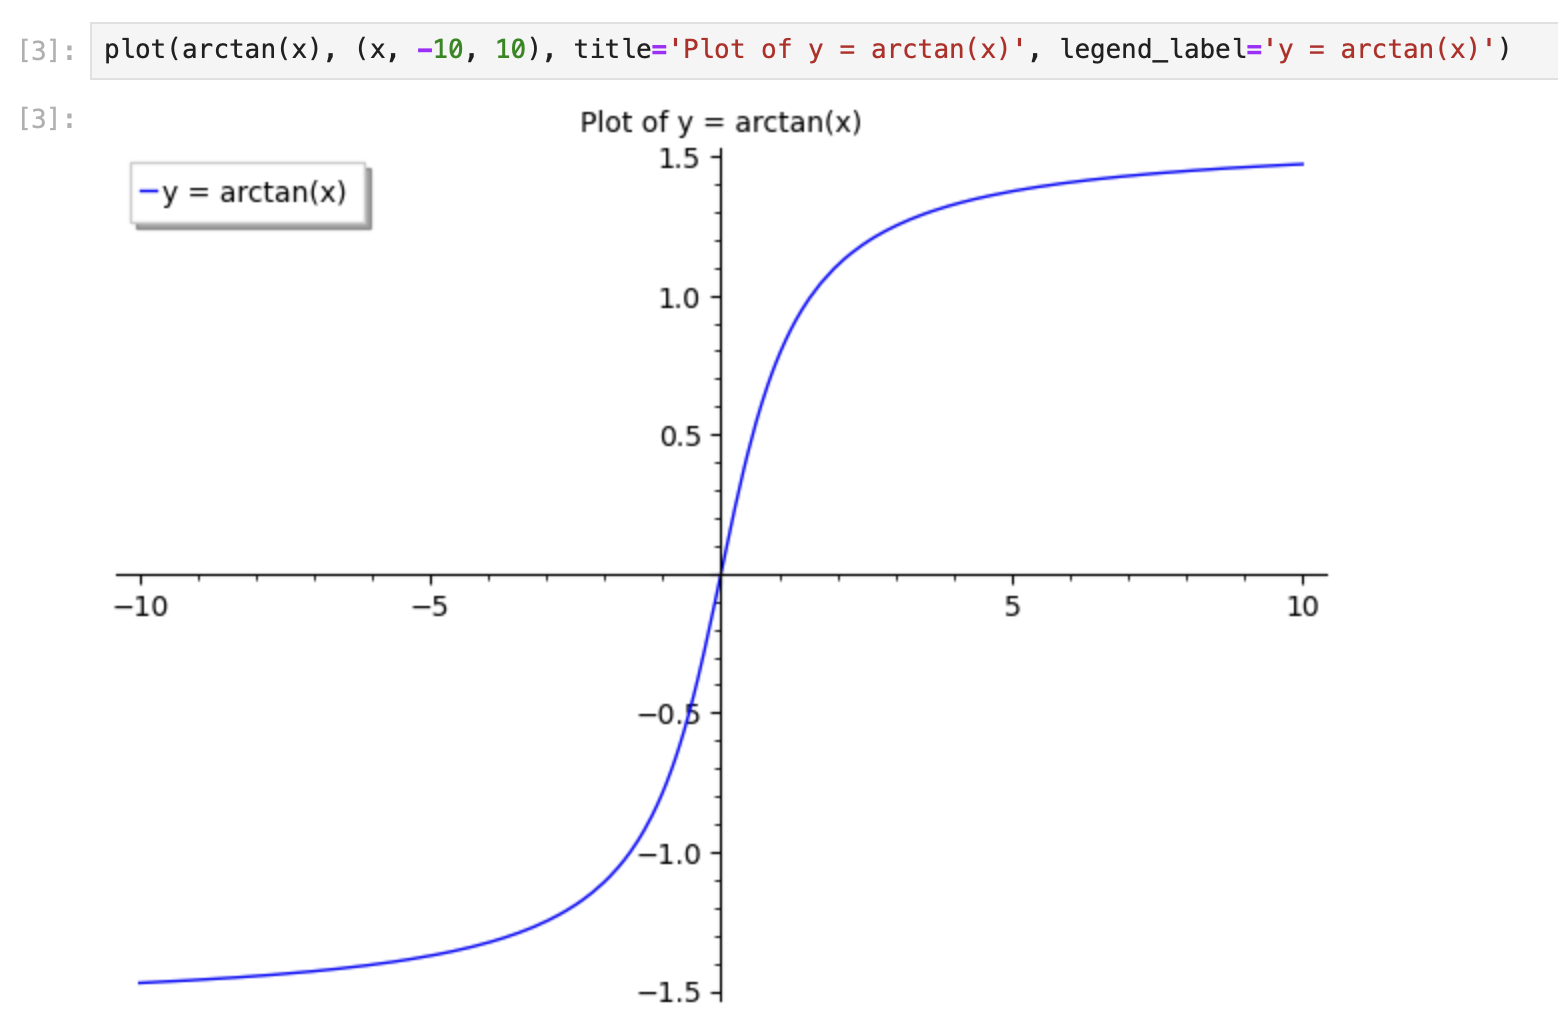
\includegraphics[height=8cm,width=15cm]{pdehw1}
   \end{minipage}
\end{center}
\end{proof}
\begin{theorem}
\begin{align}
\label{he2}
\text{ Solve }au_x+b u_y +cu=0
\end{align}
\end{theorem}
\begin{proof}
Fix 
\begin{align*}
\begin{cases}
  x'\triangleq ax+by \\
  y'\triangleq bx-ay
\end{cases}
\end{align*}
This map is clearly a diffeomorphism. Compute 
\begin{align*}
  \begin{cases}
    u_x= \frac{\partial u}{\partial x'}\frac{\partial x'}{\partial x}+\frac{\partial u}{\partial y'}\frac{\partial y'}{\partial x}=au_{x'}+bu_{y'}\\
    u_y=\frac{\partial u}{\partial x'}\frac{\partial x'}{\partial y}+\frac{\partial u}{\partial y'}\frac{\partial y'}{\partial y}=bu_{x'}-au_{y'}
  \end{cases}
\end{align*}
Plugging it back into the PDE in \myref{Equation}{he2}, we have 
\begin{align}
\label{he3}
cu+ (a^2+b^2)u_{x'}=0
\end{align}
If $c=a^2+b^2=0$, then all smooth functions are solution. If $a^2+b^2=0$ but $c\neq 0$, then clearly the only solution is $u=\tilde{0} $. If $a^2+b^2\neq 0$ but $c=0$, then $u_{x'}=\tilde{0}$, which implies $u=f(y')$ where $y'=bx-ay$ and  $f$ can be arbitrary smooth function.\\

Now, suppose $a^2+b^2\neq 0\neq c$, note that the PDE in \myref{Equation}{he3} is just an ODE of the form 
\begin{align*}
y+\frac{a^2+b^2}{c}y'=0
\end{align*}
The general solution to this ODE is 
\begin{align*}
y=Ce^{\frac{-ct}{a^2+b^2}}
\end{align*}
In other words, the general solution of the PDE in \myref{Equation}{he3} is 
\begin{align*}
u=C e^{\frac{-cx'}{a^2+b^2}}=Ce^{\frac{-c(ax+by)}{a^2+b^2}}
\end{align*}


\end{proof}
\end{document}
